\section{Opis}

Projekat se bavi sektorom prodaje u okviru poslovanje neke veleprodaje. Zaposleni u prodaje može biti komercijalista i menadžer. Komercijalista evidentira kupce i u kontaktu sa njima prima porudžbinu, recimo putem imejla. 

Porudžbina kao i svi sledeći dokumenti sadrži više stavki, stavka sadrži id porudžbine za koju je vezana i id proizvoda koji porudžbina treba da sadrži, kao i količinu.
Vrsta dokumenta u stavci odrađuje da li se radi o porudžbini, ponudi, otpremnici ili fakturi, recimo oznake su redom 1,2,3 ili 4.

Zatim komercijalista sastavlja ponudu kupcu, uz eventualno prisustvo menadžera, koji može dati popust određeni, radi uspešnije nastavka saradnje. Ponuda sadrži za razliku od porudžbine sadrži cene, i detalje posla, kao što su način ispiruke, rok isporuke, rok plaćanja, opciono kontinuitet isporuke (u sličaku da može roba iz više puta da se dostavi),... 

Ponuda može imati više otpremnica, u sličaju da je postignut dogovor oko kontinuiteta isporuke ili trenutno samo toliko možemo isporučiti. Otpremnica ne sadrži cene i ona se šalje magacinu za odvajanje robe. 

Na osnovu otpremnice se izrađuje faktura, koja naplaćuje kupcu robu koja će mu biti isporučena na osnovu otpremnice.

\subsection{Relacioni model}
\begin{itemize}
\item Zaposleni (idZaposleni, ImePrezime, DatumZaposlenja, StručnaSprema, Fukcija, UgovorenaPlata)
\item Kupac (idKupac, PIB, NazivFirme, TekućiRačun)
\item Kontakt osoba (idKupac, ImePrezime, Telefon)
\item Porudžbina (idPorudžbina, idZaposlenogKomercijalista, idKupac, DatumPorudžbine)
\item Proizvod (idProizvod, Naziv, Cena)
\item Proizvod has Proizvod (idProizvod, idProizvod1)
\item Stavka (idDokumenta, idProizvod, vrstaDokumenta, Količina)
\item Ponuda (idPonuda, idPorudžbina, idZaposleniMenadžer, DatumPonude, Cena, Popust, ProdajnaCena, Kontinuitet isporuke, Način isporuke, Rok plaćanja)
\item Otpremnica (idOtpremnica, idMagacina)
\item Otpremnica has Ponuda (idOtpremnica, idPonuda)
\item Faktura (idFaktura, idPonuda, idOtpremnica, Rok isporuke, Način isporuke)
\end{itemize}

\subsection{Uslovi}
\begin{itemize}
\item Nezavisni eniteti: Zaposleni, Kupac, Porudžbina, Ponuda, Otpremnica, Faktura
\item Agregirani entiteti: Porudžbina ,OtpremnicaHasPonuda
\item Rekurzivni odnos: ProizvodHasProizvod
\item Slabi entitet: Kontakt osoba
\end{itemize}

\clearpage

\begin{figure}[ht]
\centering
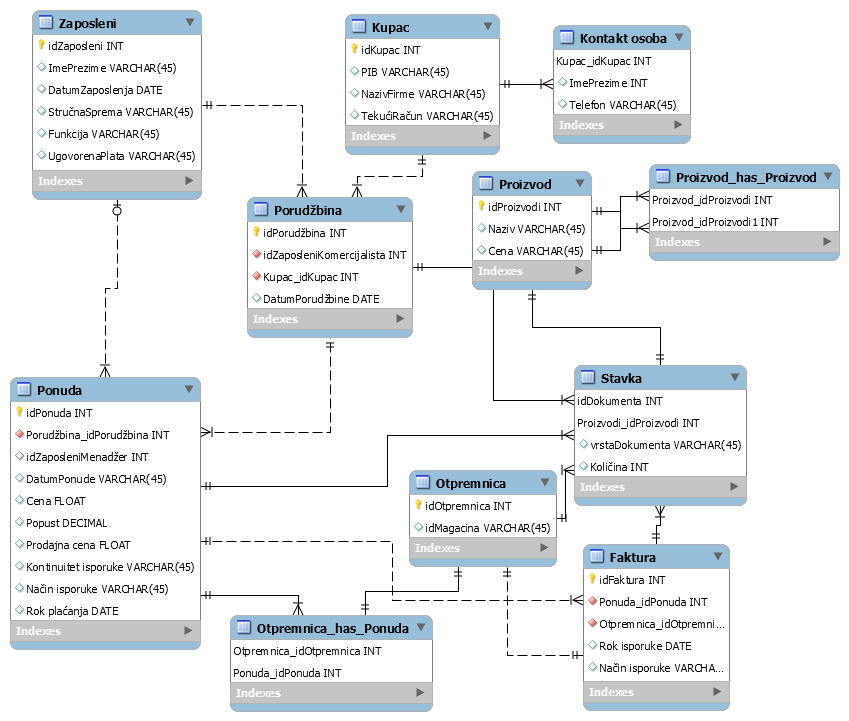
\includegraphics[width=160mm]{slike/eer.png}%
\caption{EER dijagram}
\end{figure}

\clearpage